\documentclass{article}

% Packages
\usepackage{changepage} % For adjustwidth environment
\usepackage{array}
\usepackage[utf8]{inputenc}
\usepackage{graphicx}
\usepackage{hyperref}
\usepackage{listings}
\usepackage{xcolor}
\usepackage{float}
\usepackage[margin=0.9in]{geometry} % Narrower margins
\usepackage{lipsum}
\usepackage{svg}

% Define colors for code listings
\definecolor{codegreen}{rgb}{0,0.6,0}
\definecolor{codegray}{rgb}{0.5,0.5,0.5}
\definecolor{codepurple}{rgb}{0.58,0,0.82}
\definecolor{backcolour}{rgb}{0.95,0.95,0.92}

% Code listing style
\lstdefinestyle{mystyle}{
    backgroundcolor=\color{backcolour},   
    commentstyle=\color{codegreen},
    keywordstyle=\color{magenta},
    numberstyle=\tiny\color{codegray},
    stringstyle=\color{codepurple},
    basicstyle=\ttfamily\footnotesize,
    breakatwhitespace=false,         
    breaklines=true,                 
    captionpos=b,                    
    keepspaces=true,                 
    numbers=left,                    
    numbersep=5pt,                  
    showspaces=false,                
    showstringspaces=false,
    showtabs=false,                  
    tabsize=2
}

\lstset{style=mystyle}

% Title
\title{Progetto di Reti Logiche}
\author{Matteo Arrigo}
 \date{06/03/2024} % Set the desired date here

\begin{document}

\maketitle

\section{Introduzione}

Il presente progetto è stato svolto come prova finale del corso di Reti Logiche del terzo anno di Ingegneria Informatica al Politecnico di Milano.

Il compito è progettare un’architettura hardware che soddisfi la specifica funzionale assegnata, sia in pre-sintesi sia in post-sintesi, avendo come unico vincolo non funzionale quello di assicurarsi che i ritardi di propagazione dei segnali non superino il periodo di clock assegnato (20 ns).

L’interfaccia dell’architettura è la seguente:

\begin{figure}[h]
    \centering
    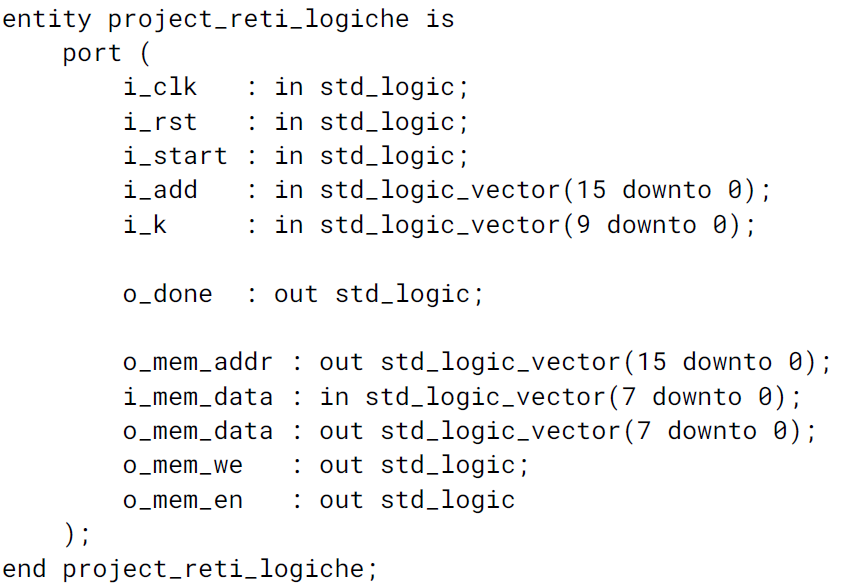
\includegraphics[width=0.5\textwidth]{specifica.png} % Replace 'example-image' with the filename of your image
    \label{fig:Specifica funzionale - Interfaccia dell'architettura}
\end{figure}

Il sistema inoltre si interfaccia con una memoria indirizzata al byte con $2^{16}$ parole da \(1\) Byte.

Le operazioni da fare in sequenza, una volta iniziate, dipendono dal valore \texttt{ADD} e \texttt{K} dati dagli ingressi \texttt{i\_add} e \texttt{i\_k}. Si deve iniziare a leggere la memoria dall’indirizzo \texttt{ADD} per un totale di 2K parole, divise in posizioni pari (da dove iniziamo a leggere), che indicano dei valori significativi, e posizioni dispari, che indicano il valore di credibilità del valore significativo precedente. Il compito del sistema è rimpiazzare i valori significativi nulli con l’ultimo valore significativo non-nullo letto, e impostare il suo valore di credibilità in base a questo. Se viene letto un valore non-nullo, il suo valore di credibilità è impostato a \texttt{31}, mentre, per ogni valore significativo nullo letto di seguito, la credibilità viene decrementata. Se la credibilità raggiunge \texttt{0}, rimane a tale valore senza essere decrementata fino alla lettura del primo valore significativo non-nullo.

Se viene letto un valore significativo nullo all’inizio della sequenza delle operazioni, e finché rimane tale, viene lasciato nullo e impostata a \texttt{0} anche la sua credibilità. Per sequenze di operazioni successive e dopo ogni reset, la logica di funzionamento è sempre la stessa.

I segnali \texttt{o\_mem\_addr}, \texttt{i\_mem\_data}, \texttt{o\_mem\_data}, \texttt{o\_mem\_we}, \texttt{o\_mem\_en} servono ad interfacciarsi con la memoria, con gli ovvi significati suggeriti dai nomi, mentre \texttt{i\_clk} è il segnale di clock che sincronizza tutti gli altri segnali. In particolare, escluso l’unico segnale asincrono \texttt{i\_rst}, tutti i segnali sono da interpretare sul fronte di salita del clock. Gli altri segnali sono:


\begin{enumerate}
    \item \textbf{i\_rst}: segnale asincrono che resetta il sistema. Si può alzare \texttt{i\_start} solo dopo aver abbassato \texttt{i\_rst}. Il funzionamento del sistema prima della prima volta in cui \texttt{i\_rst} viene portato alto non è specificato.
    \item \textbf{i\_start}: indica l’inizio delle operazioni. Rimane alto finché \texttt{o\_done} non diventa '1', dopo di che si deve abbassare. Dopo che anche \texttt{o\_done} viene abbassato, si può ricominciare un’altra sequenza di operazioni direttamente usando \texttt{i\_start}, senza dover resettare nuovamente il sistema con \texttt{i\_rst}.
    \item \textbf{i\_add}: indica il valore ADD della specifica funzionale.
    \item \textbf{i\_k}: indica il valore K della specifica funzionale.
    \item \textbf{o\_done}: segnala  la fine della sequenza di operazioni quando diventa '1'. Una volta alzato non si deve più dialogare con la memoria, e si deve abbassare dopo che \texttt{i\_start} è passato a '0'.
\end{enumerate}

Un esempio di una possibile sequenza di tali operazioni è dato, con ADD=10 e K=10 da: 

\begin{table}[htbp]
    \begin{adjustwidth}{-1.cm}{}
    \centering
    \begin{tabular}{|c|c|c|c|c|c|c|c|c|c|c|c|c|c|c|c|c|c|c|c|c|c|c|}
        \hline
        Addr & 10 & 11 & 12 & 13 & 14 & 15 & 16 & 17 & 18 & 19 & 20 & 21 & 22 & 23 & 24 & 25 & 26 & 27 & 28 & 29 & 30 & 31 \\
        \hline
        Prima & 0 & 0 & 128 & 0 & 64 & 0 & 0 & 0 & 0 & 0 & 100 & 0 & 1 & 0 & 0 & 0 & 1 & 0 & 23 & 0 & 0 & 0 \\
        Dopo & 0 & 0 & 128 & 31 & 64 & 31 & 64 & 30 & 64 & 29 & 100 & 31 & 1 & 31 & 1 & 30 & 1 & 31 & 23 & 31 & 0 & 0 \\
        \hline
    \end{tabular}
    \end{adjustwidth}
\end{table}



\section{Architettura}
Di seguito è descritta l’architettura progettata e implementata per il progetto. Il nome dei segnali fa riferimento al nome dato nel codice VHDL dell’architettura principale. Nel complesso, l’architettura è divisa in 3 moduli indipendenti tra loro e una macchina a stati che gestisce i segnali di controllo. I segnali di input/output direttamente gestiti dall’architettura sono stati evidenziati in rosso, mentre i segnali di controllo gestiti dalla FSM (quindi le uscite della FSM) sono state evidenziate in blu. I segnali verdi sono quello di reset e di clock, presenti nei registri, mentre il resto dei segnali non evidenziati sono segnali interni (corrispondenti a \texttt{signal} in VHDL). Sono stati indicati tra parentesi il numero di bit dei segnali.

I moduli architetturali di base usati sono (con riferimento al nome delle rispettive entity date in VHDL):
\begin{itemize}
    \item \textbf{mux}: un MUX standard con 2 ingressi da 16 bit, 1 uscita da 16 bit, e un bit di selezione.
    \item \textbf{reg16}: un registro sincrono (flip-flop) da 16 bit, con anche un segnale di reset asincrono e un segnale di load che abilita alla scrittura quando è alto.
    \item \textbf{addr16}: un sommatore da 16 bit implementato tramite un 16 full-adder (usato effettivamente solo come incrementatore o decrementatore).
\end{itemize}

\subsection{Modulo 1: Gestore dell'indirizzo di memoria}

\begin{figure}[htbp]
  \centering
  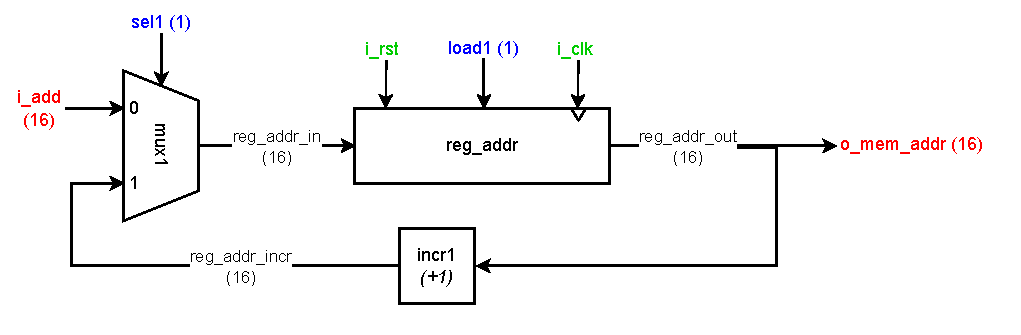
\includegraphics[width=0.8\textwidth]{modulo1.pdf}
%  \caption{Modulo 1: gestore dell'indirizzo di memoria}
  \label{fig:Modulo 1: gestore dell'indirizzo di memoria}
\end{figure}

Il bit \texttt{\textcolor{blue}{sel1}} manda in ingresso registro di \texttt{reg\_addr} il segnale \texttt{\textcolor{red}{i\_add}} (per l’inizializzazione) o l’uscita del registro stessa dopo che è stata incrementata (quindi l’uscita del modulo \texttt{incr1}, che esegue l’operazione +1). La scrittura del registro \texttt{reg\_addr} è governata dal bit \texttt{\textcolor{blue}{load1}}. L’uscita del registro rappresenta l’uscita \texttt{\textcolor{red}{o\_mem\_addr}} di tutta l’architettura.

L’implementazione in VHDL è totalmente Structural.

\subsection{Modulo 2: Gestore del numero di iterazioni}

\begin{figure}[H]
  \centering
  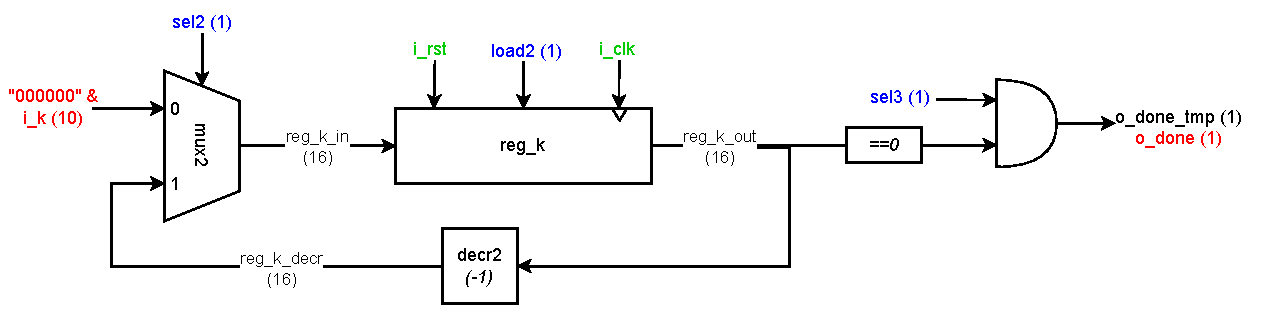
\includegraphics[width=0.82\textwidth]{modulo2.pdf}
%  \caption{Modulo 2: gestore del numero di iterazioni}
  \label{fig:Modulo 2: gestore del numero di iterazioni}
\end{figure}

Il bit \texttt{\textcolor{blue}{sel2}} manda in ingresso al registro \texttt{reg\_k} il segnale \texttt{\textcolor{red}{i\_k}} (per l’inizializzazione) o l’uscita del registro stessa dopo che è stata decrementata (quindi l’uscita del modulo \texttt{decr2}, che esegue l’operazione -1). La scrittura del registro \texttt{reg\_k} è governata dal bit \texttt{\textcolor{blue}{load2}}. Il modulo \texttt{==0} ha in uscita ‘1’ se \texttt{reg\_k\_out} è nullo, ‘0’ altrimenti, e, in AND col bit \texttt{\textcolor{blue}{sel3}}, definisce l’uscita \texttt{\textcolor{red}{o\_done}}.

L’implementazione in VHDL è mista, quasi tutta Structural esclusa una parte Behavioural (quindi un \texttt{process}) per definire l’uscita \texttt{\textcolor{red}{o\_done}} in funzione di \texttt{reg\_k\_out} e \texttt{\textcolor{blue}{sel3}}. Il segnale ausiliario \texttt{o\_done\_tmp} serve per permette la lettura di \texttt{\textcolor{red}{o\_done}} (come ingresso delle FSM), che altrimenti sarebbe solo un’uscita (non leggibile) dell’architettura.

\subsection{Modulo 3: Gestore dell'interazione con la memoria}

\begin{figure}[H]
  \centering
  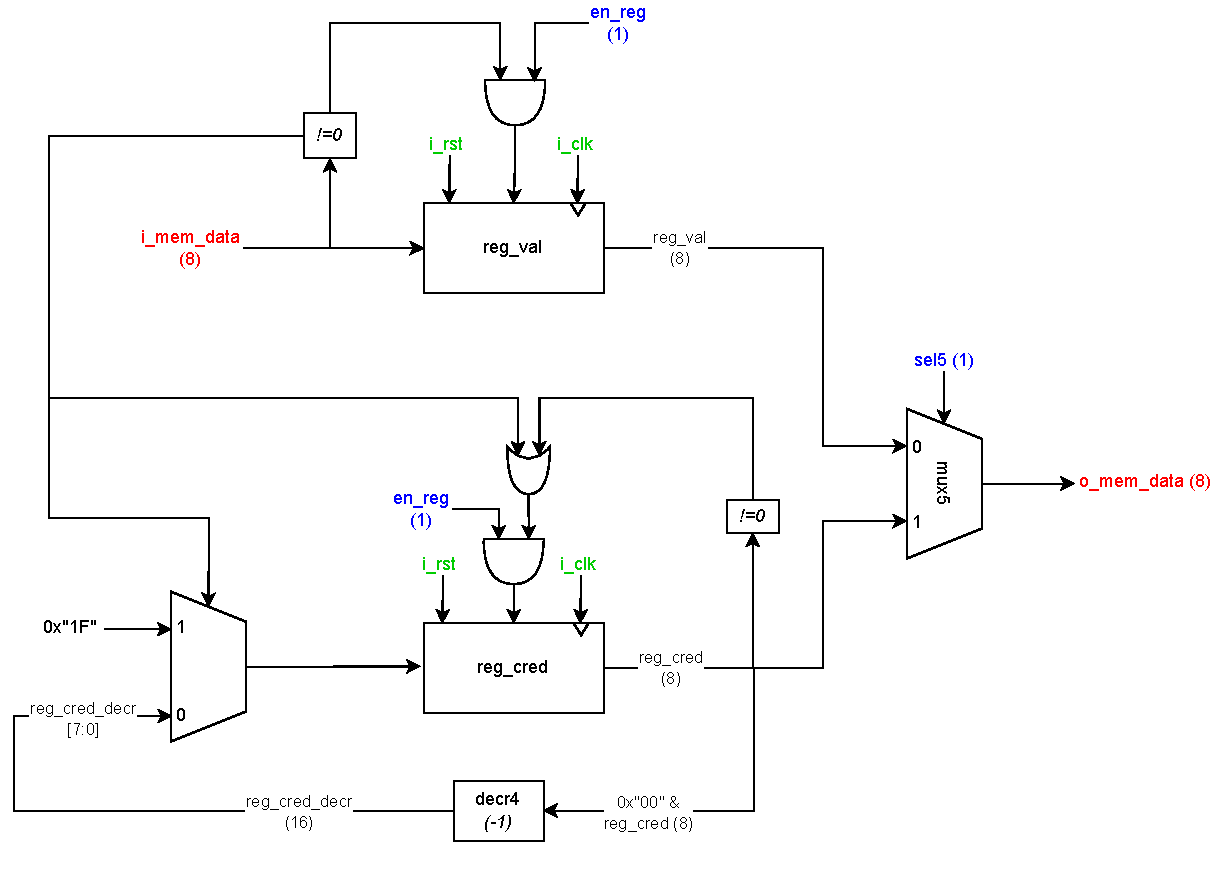
\includegraphics[width=0.95\textwidth]{modulo3.pdf}
%  \caption{Modulo 3: Gestore dell'interazione con la memoria}
  \label{fig:Modulo 3: Gestore dell'interazione con la memoria}
\end{figure}

Si possono individuare la gestione di 3 parti principali:
\begin{itemize}
    \item \textbf{Registro reg\_val}: registro che immagazzina l’ultimo valore non nullo non letto. È abilitato in scrittura se il bit \texttt{\textcolor{blue}{en\_reg}} è alto e il valore \texttt{\textcolor{red}{i\_mem\_data}} è non-nullo (serve per memorizzare il valore se è non-nullo, altrimenti viene lasciato in memoria l’ultimo non-nullo).
    \item \textbf{Registro reg\_cred}: L’ingresso è il valore 31 (base 10) o la sua uscita decrementata (quindi l’uscita di \texttt{decr4}, che esegue l’operazione -1). La scelta dell’ingresso dipende dalla nullità del segnale \texttt{\textcolor{red}{i\_mem\_data}} (se il valore letto è non-nullo, impostiamo 31 come valore di credibilità standard, altrimenti decrementiamo l’attuale credibilità). La scrittura del registro avviene se \texttt{\textcolor{blue}{en\_reg}} è alto e \texttt{\textcolor{red}{i\_mem\_data}} o l’attuale valore di credibilità sono non-nulli (in particolare dobbiamo controllare \texttt{reg\_cred!=x"00"} per non decrementare ulteriormente la credibilitàquando viene raggiunto il valore nullo).
    \item \textbf{mux5}: sceglie di mandare in uscita (\texttt{\textcolor{red}{o\_mem\_data}}) l’uscita del registro \texttt{reg\_val} o \texttt{reg\_cred} in base al bit \texttt{\textcolor{blue}{sel5}}.
\end{itemize}

 L’implementazione in VHDL è quasi completamente Behavioural, escluso l’uso dello stile Structural per gestire solo il modulo \texttt{decr4}.

\subsection{FSM}

\begin{figure}[H]
  \centering
  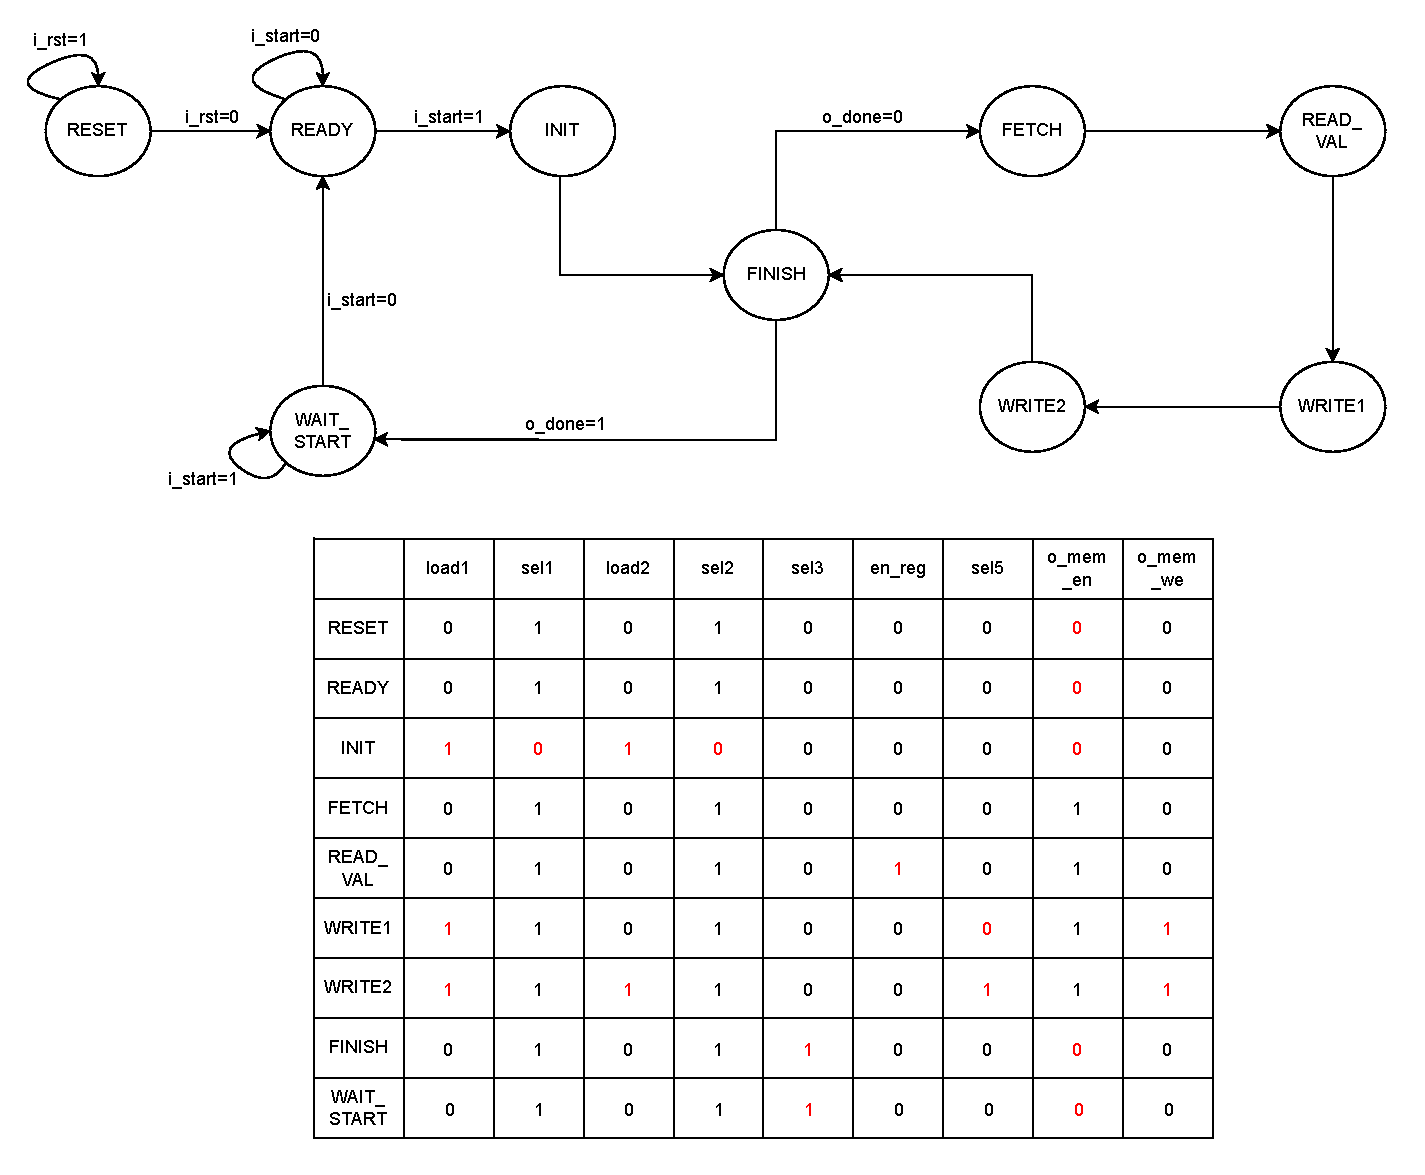
\includegraphics[width=1\textwidth, trim=0cm 11cm 0cm 0cm, clip]{modulofsm.pdf}
%  \caption{FSM}
  \label{fig:FSM}
\end{figure}

\begin{table}[htbp]
\centering
\begin{tabular}{|c|*{9}{c|}}
\hline
& load1 & sel1 & load2 & sel2 & sel3 & en\_reg& sel5 & o\_mem\_en & o\_mem\_we \\
\hline
RESET & 0 & 1 & 0 & 1 & 0 & 0 & 0 & \textcolor{red}{0} & 0 \\
\hline
READY & 0 & 1 & 0 & 1 & 0 & 0 & 0 & \textcolor{red}{0} & 0 \\
\hline
INIT & \textcolor{red}{1} & \textcolor{red}{0} & \textcolor{red}{1} & \textcolor{red}{0} & 0 & 0 & 0 & \textcolor{red}{0} & 0 \\
\hline
FETCH & 0 & 1 & 0 & 1 & 0 & 0 & 0 & 1 & 0 \\
\hline
READ\_VAL & 0 & 1 & 0 & 1 & 0 & \textcolor{red}{1} & 0 & 1 & 0 \\
\hline
WRITE1 & \textcolor{red}{1} & 1 & 0 & 1 & 0 & 0 & \textcolor{red}{0} & 1 & \textcolor{red}{1} \\
\hline
WRITE2 & \textcolor{red}{1} & 1 & \textcolor{red}{1} & 1 & 0 & 0 & \textcolor{red}{1} & 1 & \textcolor{red}{1} \\
\hline
FINISH & 0 & 1 & 0 & 1 & \textcolor{red}{1} & 0 & 0 & \textcolor{red}{0} & 0 \\
\hline
WAIT\_START & 0 & 1 & 0 & 1 & \textcolor{red}{1} & 0 & 0 & \textcolor{red}{0} & 0 \\
\hline
\end{tabular}
%\caption{Uscite della FSM}
\label{tab:Uscite della FSM}
\end{table}

La macchina a stati gestisce i segnali di controllo passando per 9 stati. È stata progettata come macchina di Moore, quindi le uscite si possono indicare su una tabella a parte in funzione solo dello stato corrente. Nella tabella sono stati evidenziate in rosso le uscite diverse da quelle di default per come è stata scritta la FSM nel codice VHDL.

Gli stati sono:
\begin{table}[H]
    \centering
%    \caption{Description of FSM States}
    \begin{tabular}{|l|p{15cm}|}
%        \hline
%        \textbf{State} & \textbf{Description} \\
        \hline
        RESET & Stato di reset della FSM, in cui rimane finché \texttt{i\_rst} non ritorna basso \\
        \hline
        READY & Attendiamo che \texttt{i\_start} sia portato alto, per iniziare la sequenza di operazioni \\
        \hline
        INIT & Impostiamo i valori iniziali dei registri \texttt{reg\_addr} e \texttt{reg\_k} per iniziare la sequenza di operazioni \\
        \hline
        FETCH & Abilitiamo la lettura in memoria per impostare \texttt{i\_mem\_data} con il valore significativo da considerare per questa iterazione \\
        \hline
        READ\_VAL & In base a \texttt{i\_mem\_data}, impostiamo i giusti valori per questa iterazione nei registri \texttt{reg\_val} e \texttt{reg\_cred} \\
        \hline
        WRITE1 & Scriviamo in memoria il valore di \texttt{reg\_val}. \newline Incrementiamo \texttt{reg\_addr} per prepararci alla scrittura del valore di credibilità \\
        \hline
        WRITE2 & Scriviamo in memoria il valore di \texttt{reg\_cred}. \newline Incrementiamo \texttt{reg\_addr} per prepararci alla prossima iterazione \newline Decrementiamo \texttt{reg\_k} per segnare l’iterazione come avvenuta \\
        \hline
        FINISH & Stato corrispondente alla fine di un’iterazione, in cui non dialoghiamo con la memoria. Se \texttt{i\_k} non è diventato 0, iniziamo una nuova iterazione da FETCH. Altrimenti, passiamo a WAIT\_START \\
        \hline
        WAIT\_START & Aspettiamo finché \texttt{i\_start} non ritorna basso \\
        \hline
    \end{tabular}
\end{table}

L’implementazione in VHDL è la classica implementazione vista anche a lezione, con 2 processi distinti per gestire la funzione di stato prossimo e di uscita.



\section{Risultati Sperimentali}
\subsection{Sintesi}

L’architettura descritta, una volta implementata in VHDL, si può sintetizzare e può essere simulata come se fosse su una vera FPGA (quella usata per la sintesi è quella proposta, l'Artix-7 FPGA xc7a200tfbg484-1), tramite la simulazione funzionale post-sintesi. In particolare possiamo accertarci di alcuni aspetti, basandoci sulla simulazione post-sintesi del testbench dato come esempio per il progetto.

Usando il comando TCL \texttt{report\_utilization},  si può notare come non siano stati sintetizzati latch, come voluto. Sono anzi generati 52 flip-flop, che il tool di sintesi ha probabilmente usato per gestire i 16 bit dei registri \texttt{reg\_addr}, \texttt{reg\_k}, gli 8 bit dei registri \texttt{reg\_val}, \texttt{reg\_cred} e 4 bit per gestire i 9 stati della FSM.

\begin{figure}[h]
    \centering
    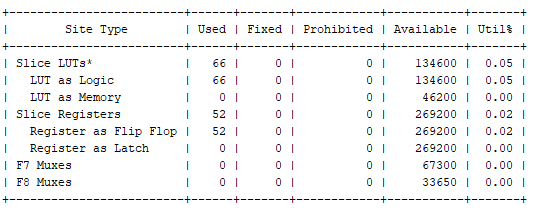
\includegraphics[width=0.5\textwidth]{report flip-flop used.png} % Replace 'example-image' with the filename of your image
    %\caption{Report utilization: Numero di flip-flop usati}
    \label{fig:Report utilization: Numero di flip-flop usati}
\end{figure}

Inoltre tramite il comando \texttt{report\_timing}, essendo presente un contraint che impone ai ritardi dei segnali di non superare il periodo di clock di 20ns, si può notare come lo slack time (tempo all’interno del periodo di clock in cui i segnali sono stabili, senza che nessuna operazione sia effettuata) sia ampiamente positivo (16.213 ns). Quindi l’architettura proposta non sembra avere problemi per quanto riguarda i ritardi dei segnali.

\begin{figure}[h]
    \centering
    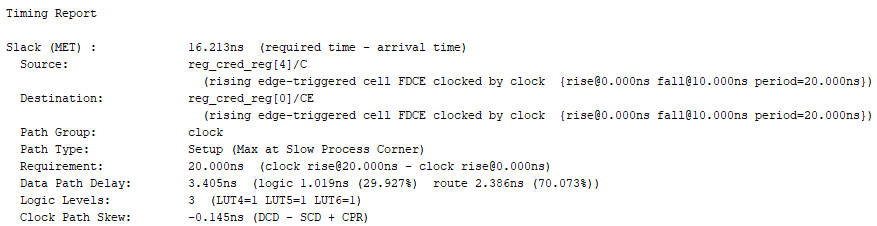
\includegraphics[width=0.8\textwidth]{report slack-time.png} % Replace 'example-image' with the filename of your image
    %\caption{Report utilization: Numero di flip-flop usati}
    \label{fig:Report timing: Slack Time}
\end{figure}


\subsection{Simulazione}

\subsubsection{Testbench 1}

K = 36, ADD = 100
\begin{table}[htbp]
    \begin{adjustwidth}{-1.75cm}{}
    \centering
%    \caption{Example Table}
    \begin{tabular}{|c|*{20}{c|}}
        \hline
        Addr & 100 & 101 & 102 & 103 & 104 & 105 & 106 & 107 & 108 & 109 & 110 & 111 & 112 & 113 & 114 & 115 & 116 & 117 & 118 & 119 \\
        \hline
        Prima & 33 & 0 & 0 & 0 & 0 & 0 & 0 & 0 & 0 & 0 & 0 & 0 & 0 & 0 & 0 & 0 & 0 & 0 & 0 & 0 \\
        Dopo & 33 & 31 & 33 & 30 & 33 & 29 & 33 & 28 & 33 & 27 & 33 & 26 & 33 & 25 & 33 & 24 & 33 & 23 & 33 & 22 \\
        \hline
        Addr & 120 & 121 & 122 & 123 & 124 & 125 & 126 & 127 & 128 & 129 & 130 & 131 & 132 & 133 & 134 & 135 & 136 & 137 & 138 & 139 \\
        \hline
        Prima & 0 & 0 & 0 & 0 & 0 & 0 & 0 & 0 & 0 & 0 & 0 & 0 & 0 & 0 & 0 & 0 & 0 & 0 & 0 & 0 \\
        Dopo & 33 & 21 & 33 & 20 & 33 & 19 & 33 & 18 & 33 & 17 & 33 & 16 & 33 & 15 & 33 & 14 & 33 & 13 & 33 & 12 \\
        \hline
        Addr & 140 & 141 & 142 & 143 & 144 & 145 & 146 & 147 & 148 & 149 & 150 & 151 & 152 & 153 & 154 & 155 & 156 & 157 & 158 & 159 \\
        \hline
        Prima & 0 & 0 & 0 & 0 & 0 & 0 & 0 & 0 & 0 & 0 & 0 & 0 & 0 & 0 & 0 & 0 & 0 & 0 & 0 & 0 \\
        Dopo & 33 & 11 & 33 & 10 & 33 & 9 & 33 & 8 & 33 & 7 & 33 & 6 & 33 & 5 & 33 & 4 & 33 & 3 & 33 & 2 \\
        \hline
        Addr & 160 & 161 & 162 & 163 & 164 & 165 & 166 & 167 & 168 & 169 & 170 & 171 & & & & & & & & \\
        \hline
        Prima & 0 & 0 & 0 & 0 & 0 & 0 & 0 & 0 & 1 & 1 & 0 & 1 & & & & & & & & \\
        Dopo & 33 & 1 & 33 & 0 & 33 & 0 & 33 & 0 & 1 & 31 & 1 & 30 & & & & & & & & \\
        \hline
    \end{tabular}
    \end{adjustwidth}
\end{table}

Questo testbench Si occupa principalmente di testare il corretto decremento di \texttt{reg\_k}, che parte da 31 (col primo valore non-nullo 33 all’indirizzo 100) e viene decrementato fino a 0, valore in cui rimane per 3 iterazioni. Inoltre si vede anche che valori non nulli agli indirizzi destinati alle credibilità non danno problemi.
Comunque, essendo il primo testbench presentato, vengono correttamente testati il comportamento generale, la gestione del comportamento basato sui segnali \texttt{i\_start} e \texttt{i\_rst}, e la corretta gestione dei segnale \texttt{o\_done}, \texttt{o\_mem\_en}, \texttt{o\_mem\_we} (per cui ci sono delle corrispondenti \texttt{assert} nel testbench)


\subsubsection{Testbench 2}

K = 7, ADD = 65522
\begin{table}[htbp]
    \begin{adjustwidth}{-1.75cm}{}
    \centering
 %   \caption{Example Table}
    \begin{tabular}{|c|*{14}{c|}}
        \hline
        Addr & 65522 & 65523 & 65524 & 65525 & 65526 & 65527 & 65528 & 65529 & 65530 & 65531 & 65532 & 65533 & 65534 & 65535 \\
        \hline
        Prima & 0 & 0 & 0 & 1 & 66 & 0 & 66 & 0 & 66 & 0 & 0 & 0 & 65 & 0 \\
        Dopo & 0 & 0 & 0 & 0 & 66 & 31 & 66 & 31 & 66 & 31 & 66 & 30 & 65 & 31 \\
        \hline
    \end{tabular}
    \end{adjustwidth}
\end{table}

Questo testbench testa il caso il cui si trovano valori significativi iniziali nulli. C’è anche il caso particolare in cui più valori significativi non-nulli consecutivi sono uguali (per cui, anche se alla fine ricompare lo stesso valore, la credibilità rimane 31). Inoltre è verificato il caso limite in cui si raggiunge la fine della memoria.

\subsubsection{Testbench 3}

K = 0, ADD = 100
\begin{table}[H]
    \begin{adjustwidth}{-1.75cm}{}
    \centering
%    \caption{Example Table}
    \begin{tabular}{|c|*{20}{c|}}
        \hline
        Addr & 100 & 101 & 102 & 103 & 104 & 105 & 106 & 107 & 108 & 109 & 110 & 111 & 112 & 113 & 114 & 115 & 116 & 117 & 118 & 119 \\
        \hline
        Prima & 33 & 0 & 33 & 0 & & & & & & & & & & & & & & & & \\
        Dopo & 33 & 0 & 33 & 0 & & & & & & & & & & & & & & & & \\
        \hline
    \end{tabular}
    \end{adjustwidth}
\end{table}

Questo testbench controlla il caso limite in cui K=0, per cui non ci devono essere iterazioni. (In questo caso, la prima volta che la FSM arriva allo stato FINISH, o\_done è già alto e quindi si va subito nello stato WAIT\_START, senza fare iterazioni).

\subsubsection{Testbench 4}

ADD1 = 100, K1 = 5; ADD2 = 110, K2 = 5
\begin{table}[H]
    \begin{adjustwidth}{-1.75cm}{}
    \centering
%    \caption{Example Table}
    \begin{tabular}{|c|*{20}{c|}}
        \hline
        Addr & 100 & 101 & 102 & 103 & 104 & 105 & 106 & 107 & 108 & 109 & 110 & 111 & 112 & 113 & 114 & 115 & 116 & 117 & 118 & 119 \\
        \hline
        Prima & 255 & 1 & 52 & 0 & 11 & 0 & 92 & 0 & 22 & 0 & 2 & 0 & 0 & 0 & 12 & 0 & 39 & 0 & 31 & 0 \\
        Dopo1 & 255 & 31 & 52 & 31 & 11 & 31 & 92 & 31 & 22 & 31 & 2 & 0 & 0 & 0 & 12 & 0 & 39 & 0 & 31 & 0 \\
        Dopo2 & 255 & 31 & 52 & 31 & 11 & 31 & 92 & 31 & 22 & 31 & 2 & 31 & 2 & 30 & 12 & 31 & 39 & 31 & 31 & 31 \\
        \hline
    \end{tabular}
    \end{adjustwidth}
\end{table}

Questo testbench controlla la corretta gestione di 2 sequenze di operazioni consecutive, senza sovrapposizione dei segmenti di memoria gestiti. La seconda sequenza è fatta partire senza prima resettare la macchina.

\subsubsection{Testbench 5}

ADD1 = 100, K1 = 8; ADD2 = 104, K2 = 8
\begin{table}[H]
    \begin{adjustwidth}{-1.75cm}{}
    \centering
%    \caption{Example Table}
    \begin{tabular}{|c|*{20}{c|}}
        \hline
        Addr & 100 & 101 & 102 & 103 & 104 & 105 & 106 & 107 & 108 & 109 & 110 & 111 & 112 & 113 & 114 & 115 & 116 & 117 & 118 & 119 \\
        \hline
        Prima & 33 & 0 & 0 & 0 & 0 & 0 & 0 & 0 & 0 & 0 & 0 & 0 & 0 & 0 & 0 & 0 & 0 & 0 & 0 & 0 \\
        Dopo1 & 33 & 31 & 33 & 30 & 33 & 29 & 33 & 28 & 33 & 27 & 33 & 26 & 33 & 25 & 33 & 24 & 0 & 0 & 0 & 0 \\
        Dopo2 & 33 & 31 & 33 & 30 & 33 & 31 & 33 & 31 & 33 & 31 & 33 & 31 & 33 & 31 & 33 & 31 & 33 & 30 & 33 & 29 \\
        \hline
    \end{tabular}
    \end{adjustwidth}
\end{table}

Questo testbench controlla la corretta gestione di 2 sequenza di operazioni consecutive, con sovrapposizione parziale dei segmenti di memoria gestiti. La seconda sequenza è fatta partire dopo il reset della macchina



\section{Conclusioni}
I testbench proposti (che comunque non sono gli unici ad essere stati usati per la fase di testing) sembrano coprire tutti i casi di interesse, senza essere ridondanti. Dato il fatto che l’architettura si comporta come aspettato sia in pre- sia in post-sintesi, è ragionevole assumere che la stessa sia stata correttamente progettata ed implementata.

Sono conscio che l’implementazione in VHDL proposta non è la più agevole da scrivere o la più immediata da leggere, essendoci diverse parti Structural e sommatori che potevano essere lasciati da implementare a VHDL, ma ho scritto l'implementazione così come è volutamente, in modo da esplorare quanto più possibile VHDL stesso secondo i metodi esposti in aula.

\end{document}
